\section{Calibcant}
\label{sec:calibcant:procedure}

A calibration run based on \cref{eq:kappa} consists of bumping the
surface with the cantilever tip to measure $\sigma_p$, measuring the
buffer temperature $T$ with a thermocouple, and measuring thermal
vibration when the tip is far from the surface to extract the fit
parameters $G_{1f}$, $f_0$, and $\beta_f$.  I've written the
\calibcant\ package to carry out this calibration procedure, building
on packages in the \pyafm\ stack (\cref{fig:calibcant:stack}).

\begin{figure}
  \tikzstack{black!20}{}
  \caption{Dependency graph for \calibcant, which shares the
    \pyafm\ stack with \unfoldprotein (\cref{fig:pyafm:stack}).  The
    only difference is that the ``brain'' module controlling the stack
    has changed from \unfoldprotein\ to
    \calibcant.\label{fig:calibcant:stack}}
\end{figure}

\subsection{Photodiode calibration}
\label{sec:calibcant:bump}

To calculate the photodiode sensitivity $\sigma_p$, we need surface
bumps with a clearly delimited contact slope.  The \calibcant\ package
uses \imint{python}|AFM.move_just_onto_surface|
(\cref{sec:pyafm:pyafm}) to position the cantilever tip a configurable
distance off the surface (\cref{sec:pyafm:h5config}).  Then
\calibcant\ uses the \pypiezo\ component (\cref{sec:pyafm:pypiezo}) to
ramp the tip towards the surface a configurable distance before
returning the tip to its original position.  The cantilever deflection
during this approach--retract cycle is analyzed to measure $\sigma_p$
(\cref{fig:calibcant:bump}).

\begin{figure}
  \begin{center}
    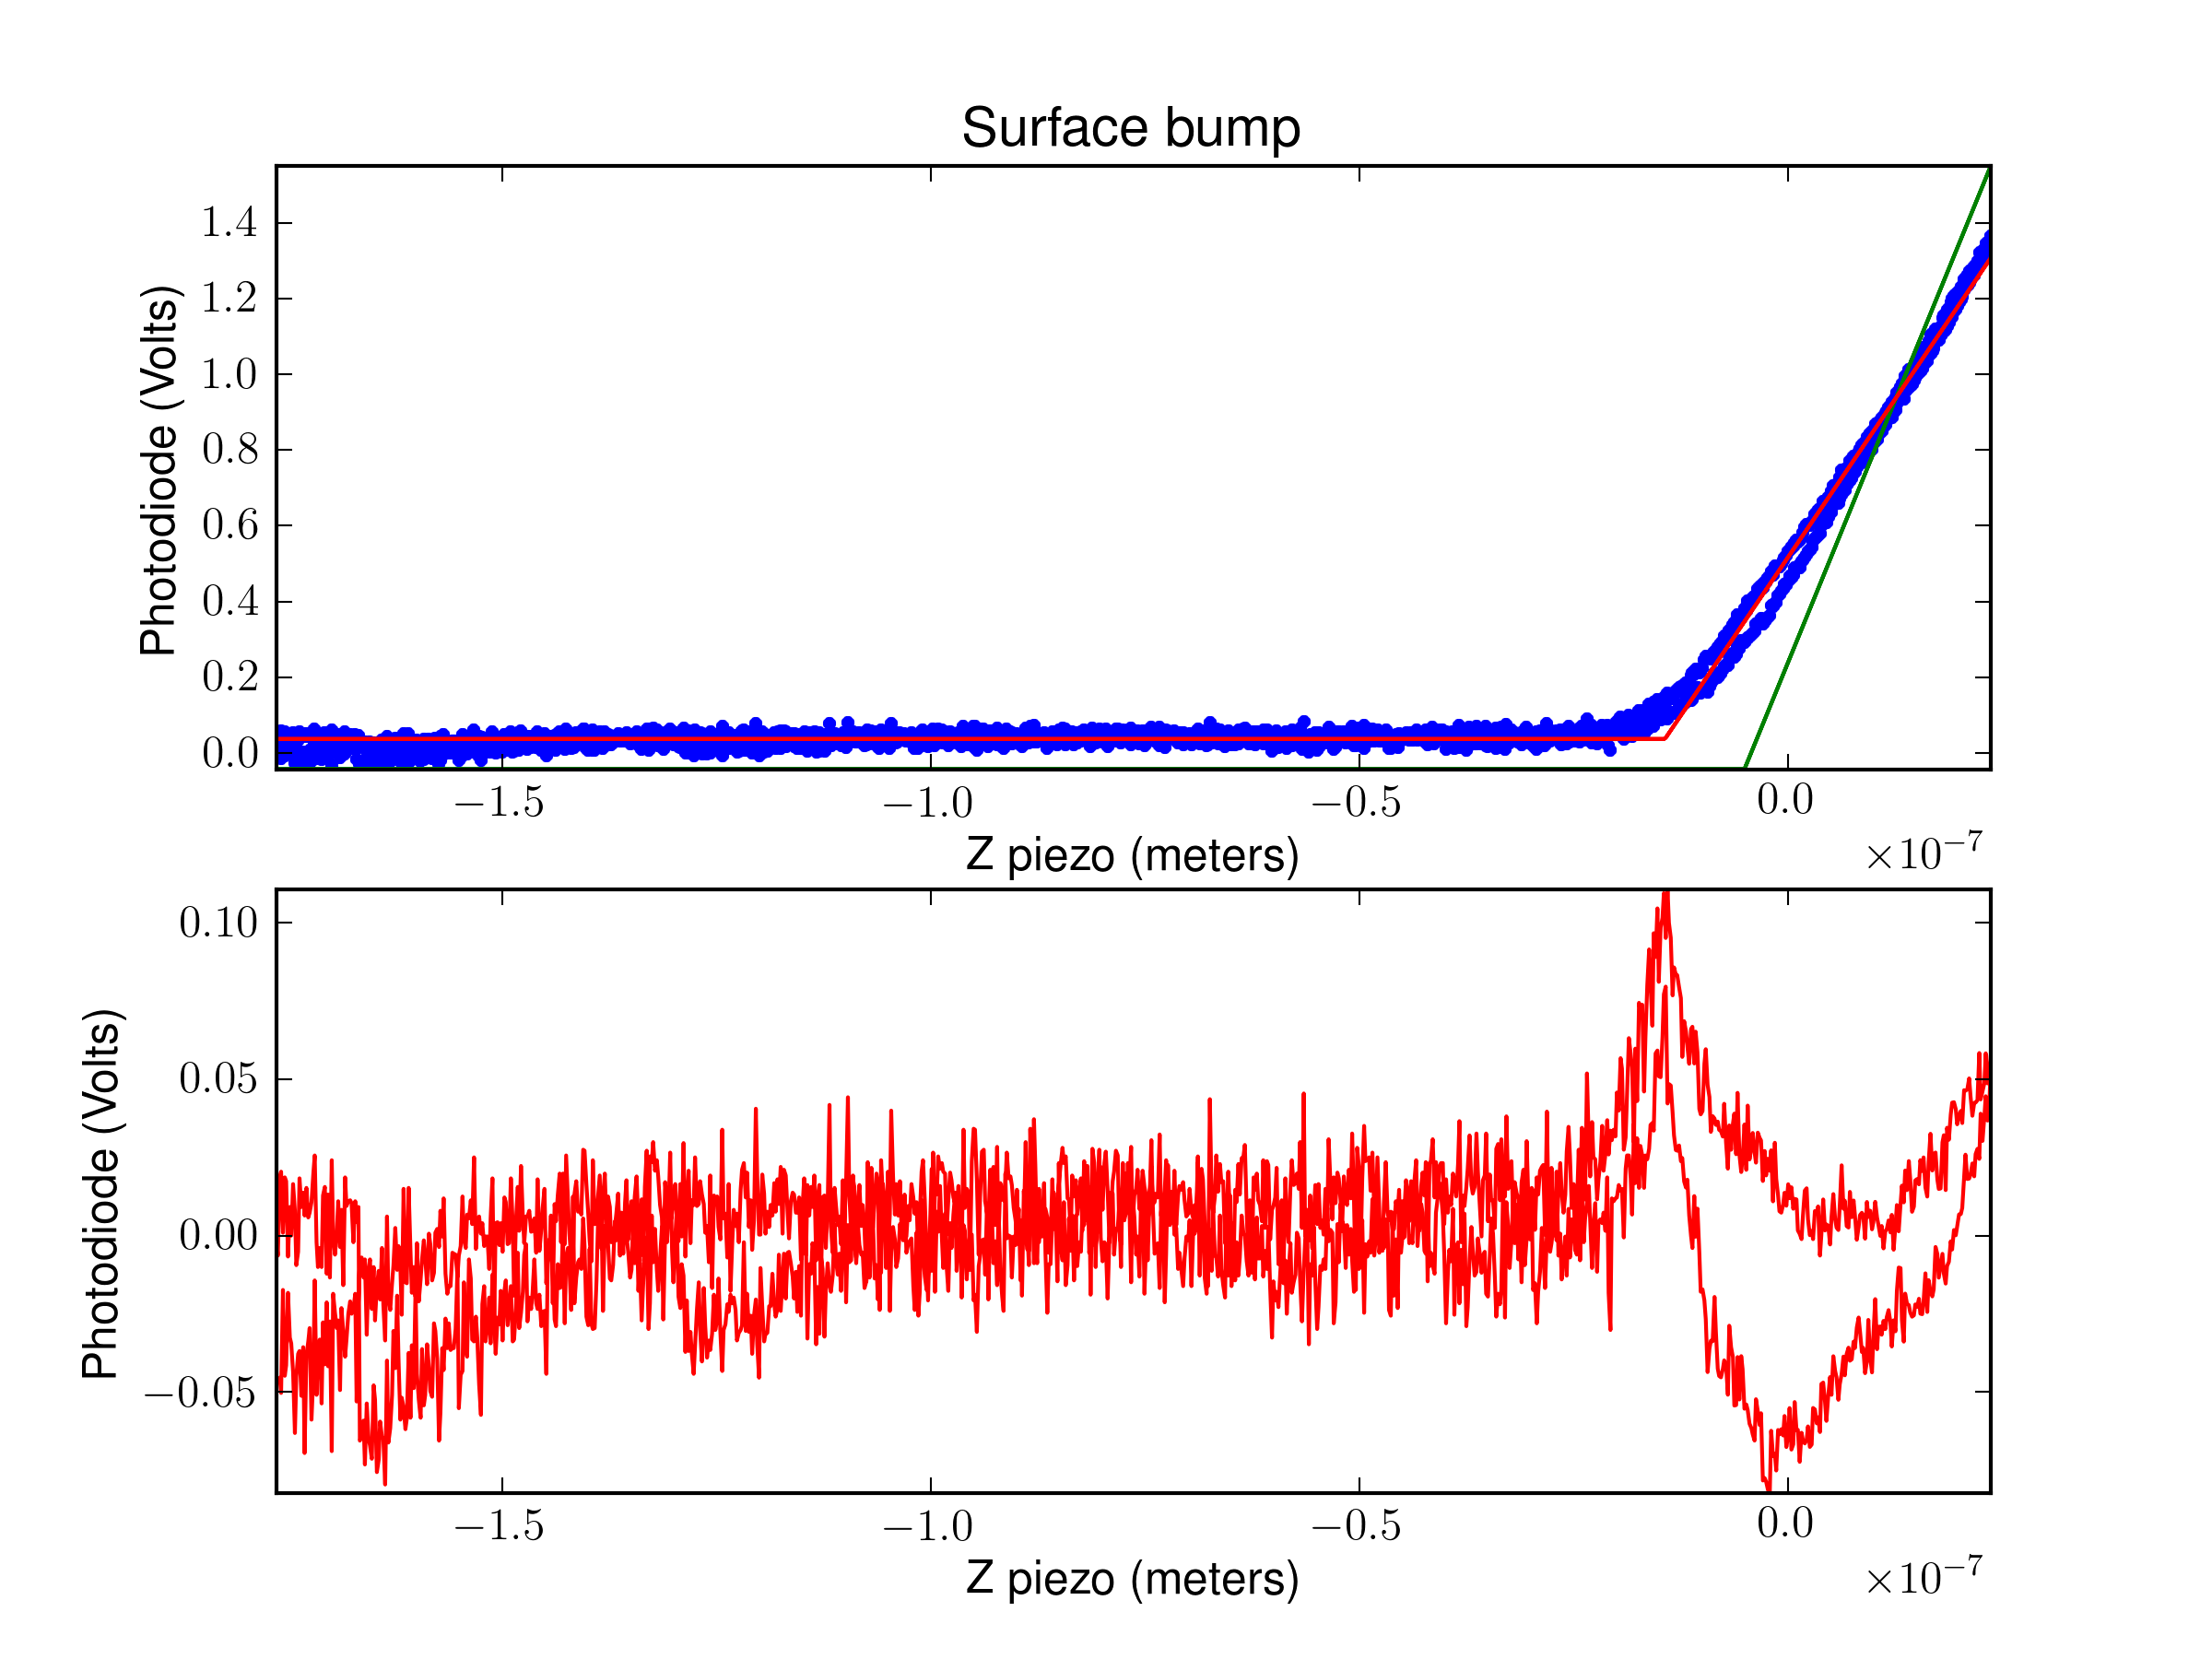
\includegraphics[width=0.8\textwidth]{figures/calibcant/bump}
    \caption{Measuring the photodiode sensitivity $\sigma_p$ by
      bumping the cantilever tip on the substrate surface.  In the
      first panel, the blue dots are experimental data, the green line
      is the heuristic guess at initial fitting parameters, and the
      red line is the optimized fit.  The second panel shows the
      residual (measured data minus modeled data) for the bump.  In
      both panels, there are two deflection measurements at each
      position, one taken during the approach phase and another taken
      during the retraction phase.  This is the first bump from the
      2013-02-07T08-20-46 calibration.\label{fig:calibcant:bump}}
  \end{center}
\end{figure}

The retraction data is analyzed using a similar approach to \pypiezo's
surface detection algorithm to extract the slope of the contact
region.  Where \pypiezo\ uses a bilinear model
(\cref{eq:bilinear-surface}), \calibcant\ uses a limited linear model:

\begin{equation}
  d(z) = \begin{cases}
      d_\text{rail}  &  z \le z_\text{rail} \\
      d_\text{kink} + \sigma_p (z - z_\text{kink})
        &  z_\text{rail} \le z \le z_\text{kink} \\
      d_\text{kink}  &  z \ge z_\text{kink}
    \end{cases}
  \label{eq:limited-linear-surface}
\end{equation}

The fitted parameters are the surface contact point $(z_\text{kink},
d_\text{kink})$ and the contact slope $\sigma_p$.  ADCs can only
digitize voltages between the rails of their power supply, and the
clipping deflection $d_\text{rail}$ is the deflection ADC's maximum
measureable voltage ($2^{16}\U{bits}$ for our 16-bit ADCs).

By explicitly modeling the clipping deflection, we avoid the need for
manual intervention when the configured approach distance is too large
for the cantilever geometry and a bump pushes too hard.  With short
cantilevers, even small tip deflection distances can generate large
laser deflection angles (\cref{fig:afm-schematic}), leading to
unmeasurable deflection voltages.  One of the unfolding pulls in
\cref{fig:pyafm:labview-comparison:many} exhibits this effect,
although it was recorded using a different stack.

An alternative approach using sinusoidal piezo oscillation in the
contact region has been proposed by \citet{materassi09}, on the
grounds that it is more reliable and easily automated than an explicit
bump and manual analysis.  While I agree that \emph{any} automated
method is likely better than manual analysis, I feel that the
difference between using an automated bump with a linear contact fit
and using an automated oscillation with a linear contact fit is likely
negligible.

\subsection{Temperature measurements}
\label{sec:calibcant:temperature}

After a series of surface bumps have been made to measure $\sigma_p$,
the stepper motor is used to move the cantilever a configurable
distance from the surface (generally $\sim30\U{$\mu$m}$).  While the
cantilever settles down after the jarring stepper motion, we measure
the buffer temperature using \pypid\ (\cref{sec:pyafm:pypid}), a
Melcor Series MTCA Thermoelectric Cooler Controller\citep{melcor}, and
a type E thermocouple\footnote{Part number 5TC-TT-E-30-72 from OMEGA
  Engineering Inc.\citep{omega}.  Breaking down the product number,
  it's a five pack of thermocouples (5TC) with perfluoroalkoxy
  insulation (TT), type E metals (chromel--constantan), number 30 AWG
  wires ($0.255\U{mm}$ diameter), in a $72\U{inch}$ length.}.  The
thermocouple is inserted through one of the ports in the AFM fluid
cell, so the thermocouple tip is in the buffer less than $3\U{mm}$
from the cantilever tip.% TODO: measure distance

\Cref{eq:kappa} depends on the \emph{absolute} temperature, so labs
without easy access to a thermocouple can probably get away with
estimating the buffer temperature.  Errors of $5\U{K}$ from an actual
temperature of around $300\U{K}$ will be within 1.7\% of the actual
value.  The effect of this error on $\kappa$ will be modest, but see
\cref{sec:calibcant:discussion:errors} for a full discussion.

\subsection{Thermal vibration}
\label{sec:calibcant:vibration}

After the temperature measurements are complete, we measure the
cantilever's thermal vibration without moving the piezo
(\cref{fig:calibcant:vibration}).  The parameters controlling these
vibrations are configurable (with \hFconfig,
\cref{sec:pyafm:h5config}), but the default values are:

\begin{description}
  \item[frequency] The sampling frequency, which defaults to
    $50\U{kHz}$.  This value gives a Nyquist frequency of $25\U{kHz}$,
    which is well above our resonant cantilever frequencies
    ($\sim5\U{kHz}$ in the buffer).
  \item[sample time] The acquisition time in seconds.  This is rounded
    up as required so the number of samples will be an integer power
    of two for efficient Fourier transformation.  It defaults to
    $1\U{s}$.
  \item[model] The vibration model.  This selects the fitting method
    for extracting the variance $\avg{V_p(t)^2}$.  By default,
    \cref{eq:psd-Vp} is used, but you can add the constant offset
    (discussed below) or use the na\"{\i}ve
    $\avg{V_p(t)^2}=\sum(V_p^2)/N$.
  \item[minimum fit frequency] The low-frequency end of the
    \PSD\ usually has a good deal of noise due to detector drift or
    background (non-cantilever) vibrations.  This parameter allows
    you to select a window of the \PSD\ for fitting that excludes the
    troublesome low-frequency region.  It defaults to $500\U{Hz}$.
  \item[maximum fit frequency] For completeness, you can also set a
    high-frequency cutoff, although I've never had to use this
    parameter.
  \item[chunk-size, overlap, \ldots] Assorted parameters for Fourier
    transforms used to compute the \PSD.
\end{description}

\begin{figure}
  \begin{center}
    \subfloat[][]{\label{fig:calibcant:vibration:offset}
      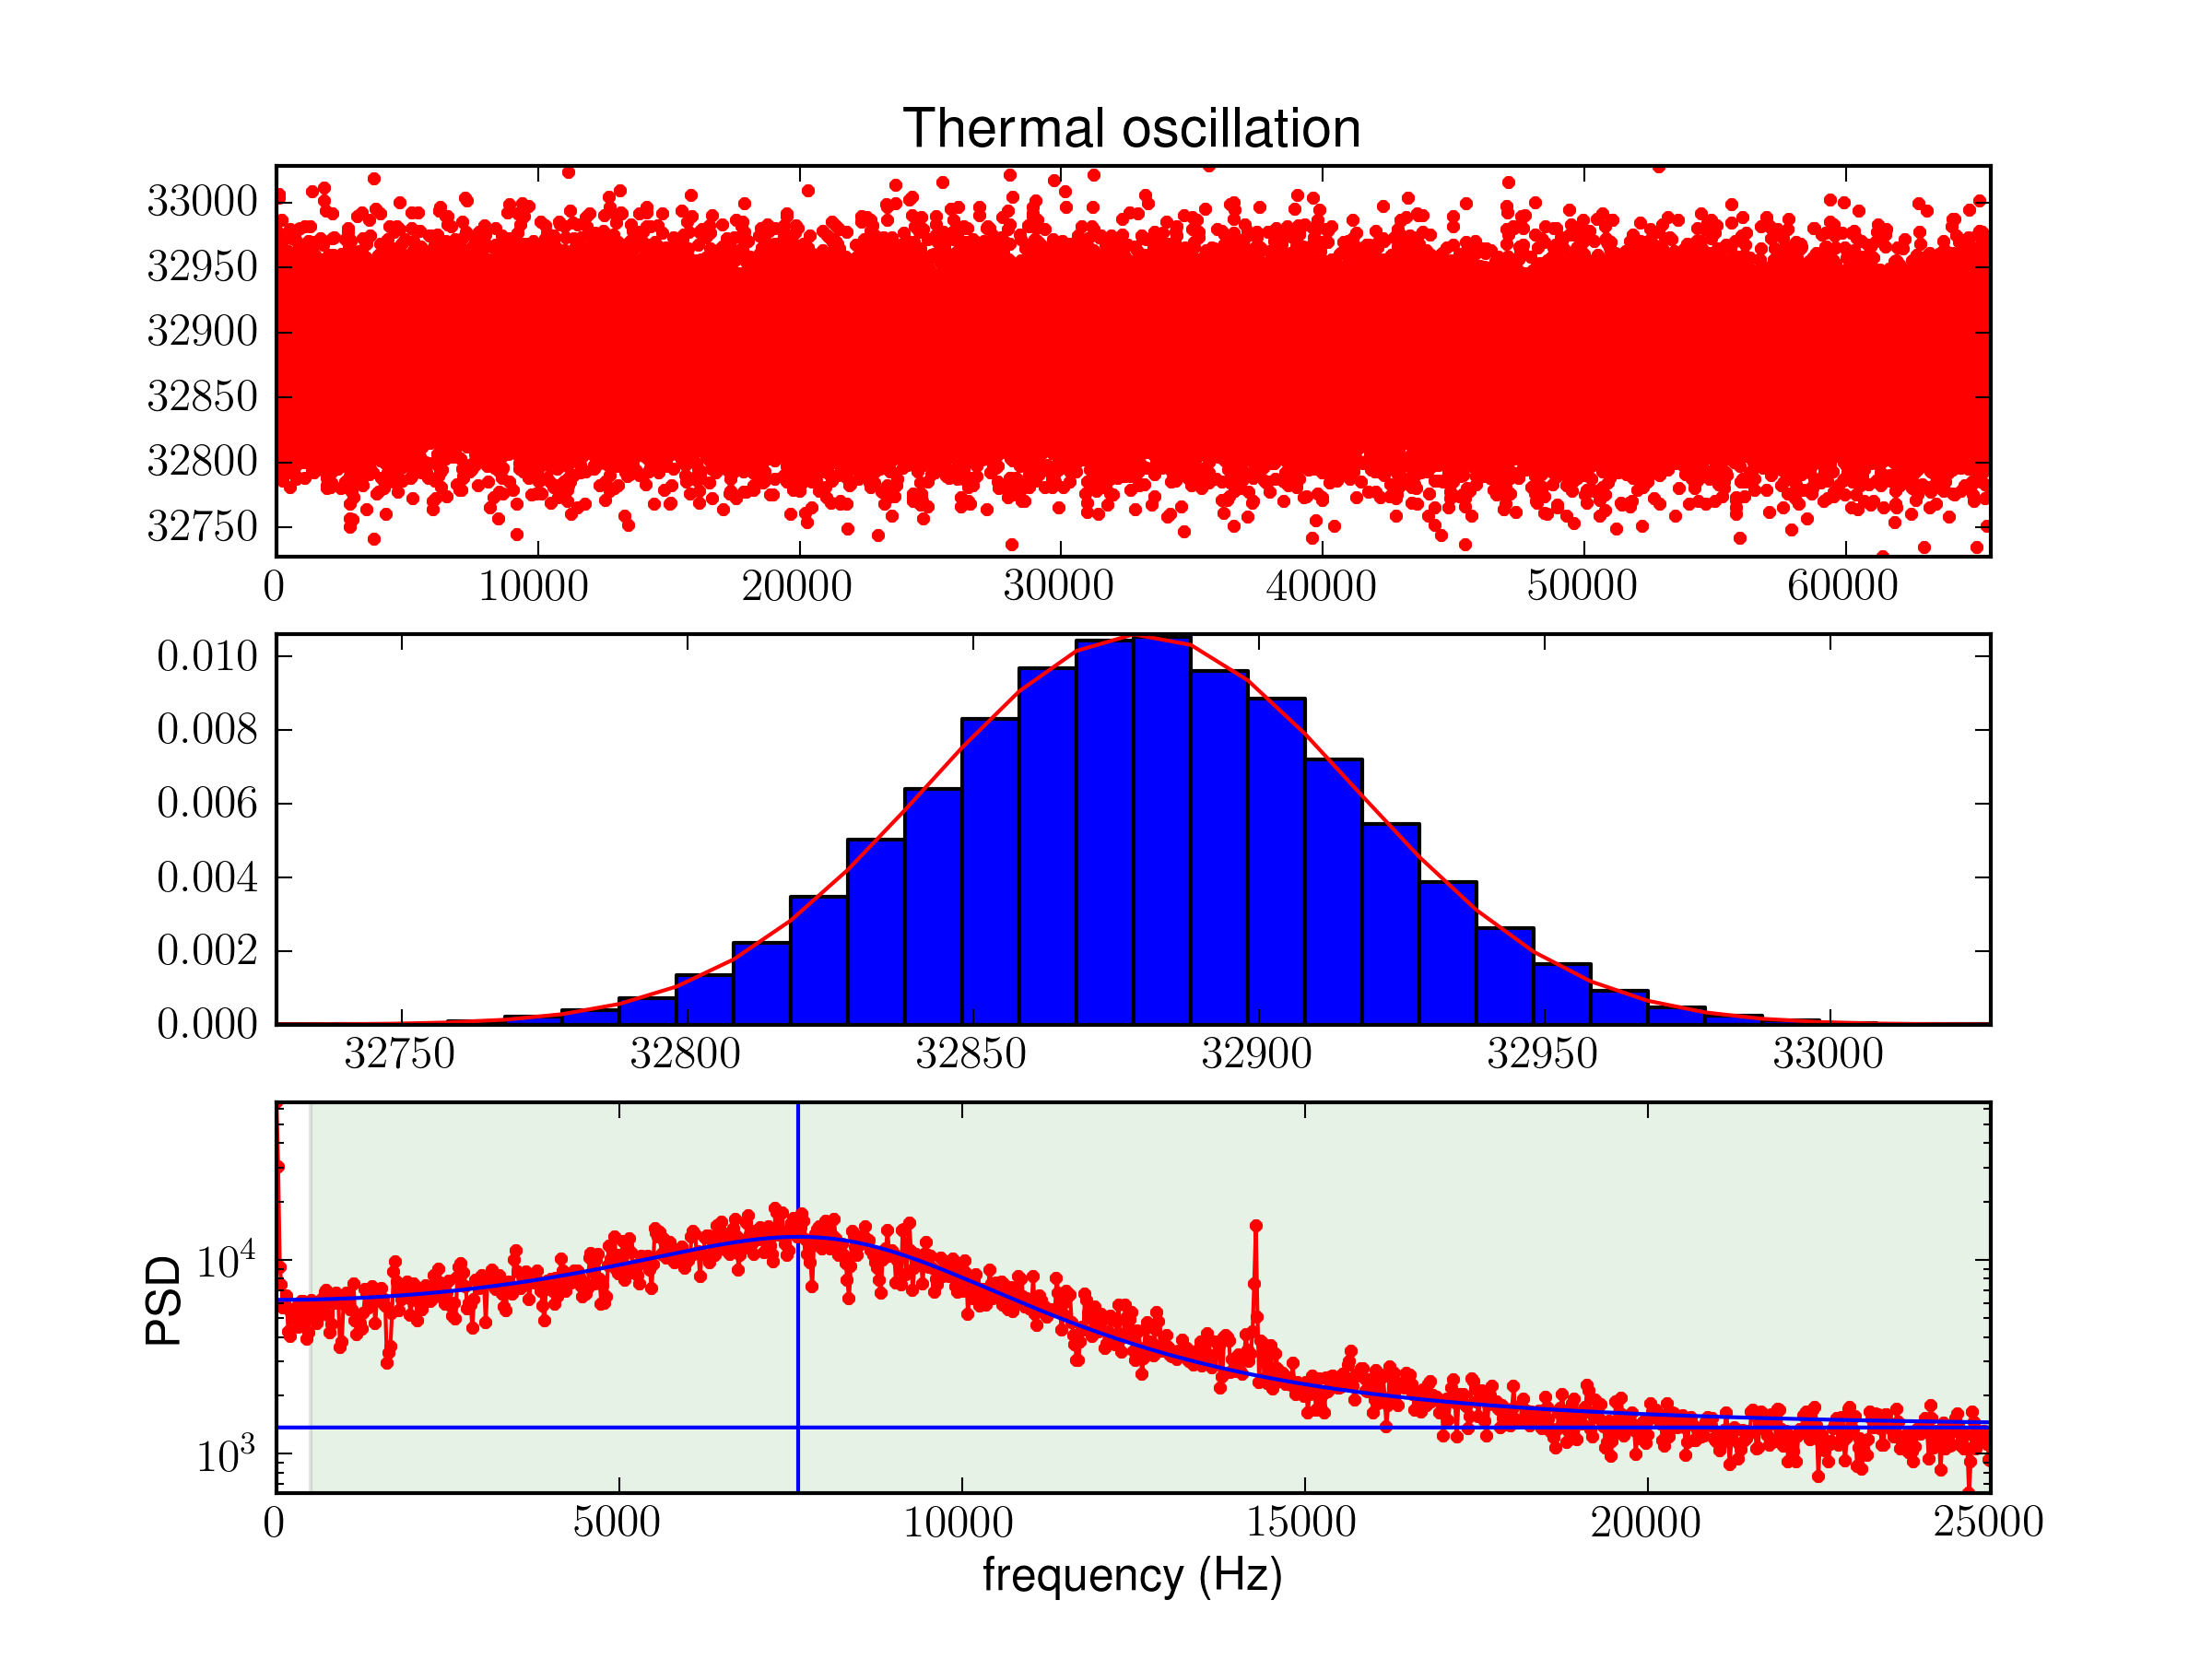
\includegraphics[width=0.8\textwidth]{figures/calibcant/vibration}}
    \caption{\protect\subref{fig:calibcant:vibration:offset}Measuring
      the cantilever's thermal vibration.  The top panel shows the raw
      time series data in bins, the middle panel shows the
      distribution of bin values with a Gaussian fit, and the bottom
      panel shows the $\PSD_f(V_p,f)$ with a fit following
      \cref{eq:psd-Vp-offset}.  The constant offset $P_{0f}$, drawn as
      the horizontal line in the third panel, accounts for white noise
      in the measurement circuit\citep{burnham03}.  The vertical line
      marks the peak frequency $f_\text{max}$
      (\cref{eq:peak-frequency}).  Only data in the blue region was
      used when computing the best fit.  This is the first vibration
      from the 2013-02-07T08-20-46 calibration, yielding a fitted
      variance $\avg{V_p(t)^2}=96.90\pm0.99\U{mV$^2$}$.  The narrow
      spike around $14.3\U{kHz}$ is not due to the cantilever's
      thermal vibration, and rejecting noise like this is the reason
      we use a frequency-space fit to calculate the thermal deflection
      variance.
      \label{fig:calibcant:vibration}}
  \end{center}
\end{figure}

\begin{figure}
  \ContinuedFloat
  \begin{center}
    \subfloat[][]{\label{fig:calibcant:vibration:no-offset}
      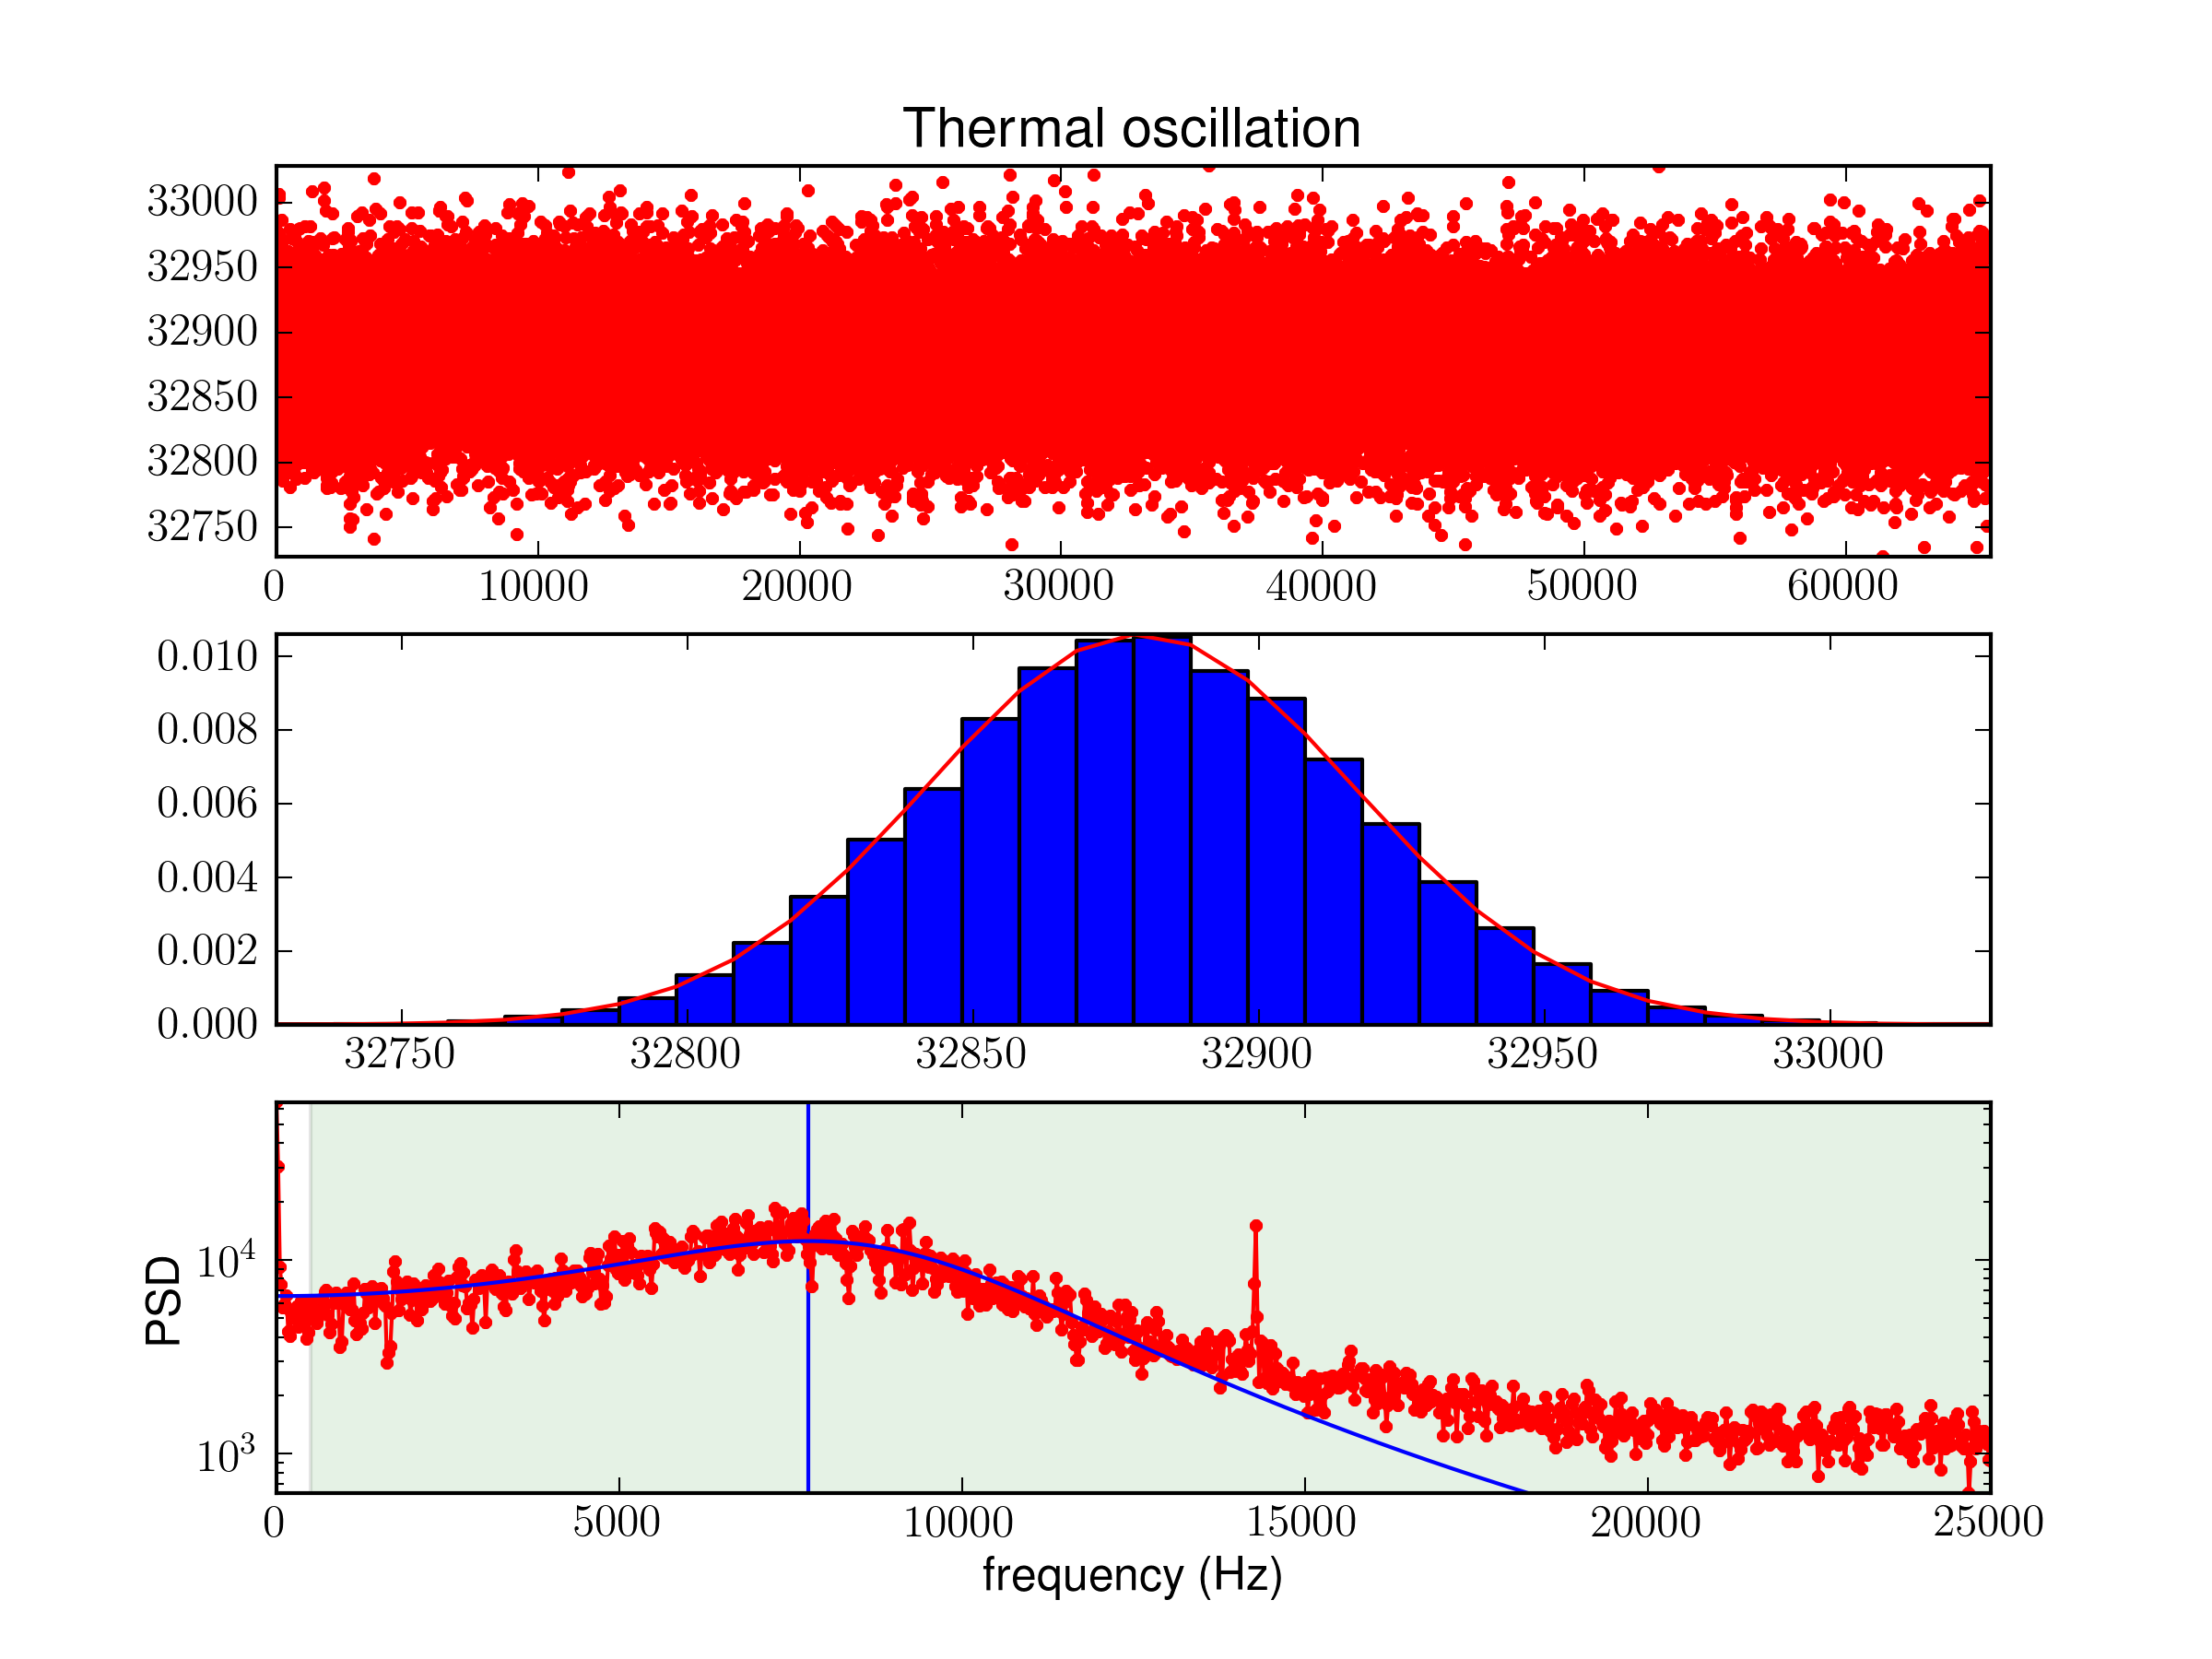
\includegraphics[width=0.8\textwidth]{figures/calibcant/vibration-no-offset}}
    \caption{\protect\subref{fig:calibcant:vibration:no-offset}This is
      the same data as in
      \protect\subref{fig:calibcant:vibration:offset} fit with
      \cref{eq:psd-Vp}, yielding a fitted variance
      $\avg{V_p(t)^2}=120.92\pm0.90\U{mV$^2$}$.  The third panel is
      very similar to figure 2 in \citet{florin95}, but they do not go
      into further detail on the method or model.  They may be fitting
      their data to \cref{eq:lorentzian}, see
      \cref{sec:calibcant:lorentzian}.  Another similar figure is in
      \citet{hutter93}.}
  \end{center}
\end{figure}

\Cref{eq:psd-Vp} decreases for large frequencies, but the measured
\PSD\ levels out (\cref{fig:calibcant:vibration:no-offset}).  I
attribute this to background white noise in the measurement circuit,
and not due to cantilever oscillation.  To avoid artificially
inflating the estimated $\avg{V_p(t)^2}$, I created an alternative
model for $\PSD_f(V_p,f)$ that adds a frequency-independent offset
$P_{0f}$\citep{burnham03}.

\begin{equation}
  \PSD_f(V_p, f) = \frac{G_{1f}}{(f_0^2-f^2)^2 + \beta_f^2 f^2} + P_{0f} \;.
  \label{eq:psd-Vp-offset}
\end{equation}

Plots of \cref{eq:psd-Vp-offset} fits look better than
\cref{eq:psd-Vp} fits (\cref{fig:calibcant:vibration}), but the
significance on the variance calculated with
\cref{eq:avg-Vp-Gone-f} depends on the amount of background noise
in the vibration data.  With over an order of magnitude difference
between the power of the damped harmonic oscillator peak and the
background noise, the effect of $P_{0f}$ will be small.  With noisier
setups, removing the white background noise can lead to a significant
difference.  The fitted variance $\avg{V_p(t)^2}$ of my
2013-02-07T08-20-46 data shifts from $120.92\pm0.90\U{mV$^2$}$ using
\cref{eq:psd-Vp} to $96.90\pm0.99\U{mV$^2$}$ using
\cref{eq:psd-Vp-offset}, a 20\% decrease.  The calculated spring
constant increases from $43.3\pm{2.1}$ to $54.1\pm2.7\U{mN/m}$, a 25\%
increase.  Changes of this magnitude are important for accurate
unfolding force calibration.
